\documentclass[aps,prd,twocolumn,superscriptaddress,floatfix]{revtex4-2}

\usepackage{amsmath,amssymb}
\usepackage{graphicx}
\usepackage{hyperref}
\usepackage{booktabs}
\usepackage{siunitx}
\usepackage{xcolor}

\graphicspath{{figures/}}

\begin{document}

\title{Computational search for emergent spacetime geometry from
cellular automata on dynamic graphs}

\author{Marco Narcisi}
\email{mnarc123@pm.me}
\affiliation{Independent Researcher, Castellalto, Abruzzo, Italy}

\date{\today}

\begin{abstract}
We present \textsc{Discretum}, a computational framework for searching
local cellular automaton rules on dynamic graphs whose evolved geometry
may reproduce features of spacetime.
A parametric rule with 14 tuneable parameters governs state transitions
and topological moves on an initially four-dimensional hypercubic lattice.
We optimise using CMA-ES and genetic algorithm against a multi-component
fitness function measuring Hausdorff dimension, Ollivier--Ricci curvature,
spectral dimension, and connectivity.

The best rule produces graphs with Hausdorff dimension rising from
$d_H = 3.09 \pm 0.01$ at $N\!=\!256$ to $d_H = 4.65$ at $N\!=\!4096$
(connected runs only); power-law extrapolation yields
$d_H(\infty) = 4.71 \pm 0.04$, systematically exceeding the target by
${\sim}18\%$.
However, three significant failures are identified:
(i)~connected fraction drops from 100\% ($N\!=\!256$) to 5\%
($N\!=\!4096$), so the rule is not thermodynamically stable;
(ii)~spectral dimension remains $d_s \lesssim 1$ for \emph{both}
evolved and bare lattices at all accessible sizes, dominated by
finite-size saturation;
(iii)~mean curvature converges to
$\langle\kappa\rangle = -0.34 \pm 0.006$ (hyperbolic, not flat).
Comparison with causal dynamical triangulations, where $d_s \to 4$
emerges with causal constraints, identifies the absence of causality
as the critical missing ingredient.
The framework is released as open-source software.
\end{abstract}

\maketitle

%% ════════════════════════════════════════════════════
\section{Introduction}
\label{sec:intro}
%% ════════════════════════════════════════════════════

A central question in quantum gravity is whether smooth spacetime
geometry can emerge from fundamentally discrete, pre-geometric
structures~\cite{Loll2019,Ambjorn2012}.  Several programmes
explore this idea.  Causal dynamical triangulations
(CDT)~\cite{Ambjorn2004,Ambjorn2005} demonstrate that
four-dimensional de~Sitter-like spacetime arises from a path
integral over simplicial geometries when a causal (foliation)
constraint is imposed.  Crucially, removing this constraint
---as in Euclidean dynamical triangulations (EDT)---yields
crumpled or branched-polymer phases with no extended
geometry~\cite{Ambjorn2012}, underscoring the role of
causal structure.  Causal set
theory~\cite{Bombelli1987,Surya2019}, spin foams~\cite{Perez2013},
and Wolfram's physics project~\cite{Wolfram2020} approach the
problem from different angles.

In this work we take an explicitly computational, bottom-up approach:
we define a parametric cellular automaton on a dynamic graph and use
metaheuristic optimisation to \emph{search} for local rules that
produce emergent geometry.  The central question is: \emph{can simple
local rules, without causal structure, generate graphs with
four-dimensional manifold-like geometry?}

Our answer is nuanced.  The best rule found achieves the correct
Hausdorff dimension scaling but fails on spectral dimension,
curvature, and large-scale connectivity.  This negative result is
itself informative: it provides quantitative evidence that acausal
local dynamics on graphs are insufficient for emergent spacetime,
supporting the theoretical arguments for the necessity of causal
structure~\cite{Ambjorn2004,Loll2019}.

The contributions of this paper are threefold:
\begin{enumerate}
\item \textbf{Framework.}  A validated, open-source framework
  (\textsc{Discretum}) for systematic computational search over
  discrete geometry models, including GPU-accelerated observables
  and ensemble diagnostics.
\item \textbf{Negative result.}  Quantitative constraints on what
  14-parameter acausal rules can and cannot achieve: correct $d_H$
  scaling but anomalous $d_s$, hyperbolic curvature, and
  connectivity instability at large~$N$.
\item \textbf{Analysis.}  Finite-size scaling with bootstrap
  extrapolation, multiscale spectral analysis with CDT comparison,
  and parameter--fitness correlations identifying the dominant
  topological dynamics.
\end{enumerate}

The paper is organised as follows.
Section~\ref{sec:model} defines the model and observables.
Section~\ref{sec:validation} validates the measurement code on
known geometries.
Section~\ref{sec:results} presents search and scaling results.
Section~\ref{sec:discussion} discusses successes, failures,
comparison with CDT, and future directions.
Section~\ref{sec:conclusions} summarises.


%% ════════════════════════════════════════════════════
\section{Model and methods}
\label{sec:model}
%% ════════════════════════════════════════════════════

\subsection{Dynamic graph cellular automaton}

The state at discrete time~$t$ is a graph $G_t = (V_t, E_t)$ where
each node $i \in V_t$ carries a state $s_i \in \{0,1,2\}$.  The
initial condition is a $d$-dimensional hypercubic lattice of
side~$L$, so $|V_0| = L^d$.

At each time step, two operations are applied:

\paragraph{State update.}
Node~$i$ in state~$a$ transitions to state~$b$ with probability
\begin{equation}
  P(a \to b \mid \mathbf{n}_i) = \frac{e^{\theta_{ab}}}
    {\sum_{c} e^{\theta_{ac}}} \,,
\end{equation}
where $\boldsymbol{\Theta}_{\mathrm{state}} = (\theta_{ab})$ is a
$3 \times 3$ matrix of raw logits and $\mathbf{n}_i$ encodes the
neighbourhood composition.

\paragraph{Topological moves.}
Five operations are attempted with probabilities
$p_k = \sigma(\theta_k^{\mathrm{topo}})$ (logistic sigmoid):
edge addition ($p_{\mathrm{add}}$, connecting nodes at
graph distance~2),
edge removal ($p_{\mathrm{rm}}$),
rewiring ($p_{\mathrm{rw}}$),
node splitting ($p_{\mathrm{sp}}$), and
node merging ($p_{\mathrm{mg}}$).

The full parameter vector
$\boldsymbol{\theta} \in \mathbb{R}^{14}$ concatenates
$\boldsymbol{\Theta}_{\mathrm{state}}$ (9~parameters) and
$\boldsymbol{\theta}^{\mathrm{topo}}$ (5~parameters).

\subsection{Geometric observables}
\label{sec:observables}

\paragraph{Ollivier--Ricci curvature.}
For an edge $(i,j)$, the curvature is
$\kappa(i,j) = 1 - W_1(\mu_i, \mu_j) / d(i,j)$, where $W_1$ is
the Wasserstein-1 distance between uniform measures $\mu_i$, $\mu_j$
on the neighbourhoods of $i$ and $j$~\cite{Ollivier2009,Lin2011}.
We compute $W_1$ via the successive shortest paths algorithm for
min-cost flow.  The mean curvature
$\langle\kappa\rangle$ is estimated by sampling 300 random edges.

\paragraph{Hausdorff dimension.}
From the volume growth function $N(r) = |\{j : d(i,j) \leq r\}|$
averaged over 30 random sources, we fit $N(r) \sim r^{d_H}$ in the
scaling regime $r \in [2, R_{\max}/2]$.

\paragraph{Spectral dimension.}
The return probability $P(t)$ of a random walk yields the effective
spectral dimension at diffusion time~$t$,
\begin{equation}
  d_{\mathrm{eff}}(t) = -2\,\frac{d\ln P}{d\ln t} \,.
\end{equation}
On a $d$-dimensional manifold, $d_{\mathrm{eff}}(t) \to d$ in the
intermediate regime $1 \ll t \ll N^{2/d}$.  We use a plateau-finding
estimator (v2) that identifies the widest window of stable
$d_{\mathrm{eff}}$, following Ambj{\o}rn
\emph{et al.}~\cite{Ambjorn2005}.  On finite graphs, $P(t) \to 1/N$
as $t \to \infty$, so $d_{\mathrm{eff}} \to 0$.  For the graph sizes
accessible here ($N \le 4096$), this saturation is severe: a bare
$5^4$ lattice yields $d_s \approx 0.6$ instead of $d_s = 4$
(Sec.~\ref{sec:validation}).  We therefore focus on relative
comparisons between evolved and bare lattices rather than absolute
$d_s$ values.

\subsection{Fitness function (version~3)}
\label{sec:fitness}

The fitness function used in the 4D campaign is
\begin{equation}
  F = -\sum_i w_i \, f_i^2 - P_{\mathrm{conn}} -
      P_{\mathrm{density}} - P_{\mathrm{degrad}} \,,
\label{eq:fitnessv3}
\end{equation}
with squared penalties:
$f_H = |d_H - d^*|$ (Hausdorff),
$f_\kappa = |\langle\kappa\rangle|$ (curvature),
$f_s = |d_s - d^*|$ (spectral--Hausdorff concordance),
$f_{\mathrm{stab}} = |\ln(N/N_0)|$ (stability),
$f_{\mathrm{reg}} = \mathrm{CV}(k)$ (regularity).
Weights are $(w_H, w_\kappa, w_s, w_{\mathrm{stab}},
w_{\mathrm{reg}}) = (2,\, 1.5,\, 1,\, 0.5,\, 0.3)$.
A fixed connectivity penalty $P_{\mathrm{conn}} = 10 \times
n_{\mathrm{comp}}$ is applied to disconnected graphs.
Density and degradation penalties prevent over-densification and
ensure the evolved graph improves on the bare lattice baseline.

\subsection{Optimisation}
\label{sec:optimisation}

We compared CMA-ES ($\sigma_0 = 0.5$, 500~generations) and a
tournament-selection GA (population 40, 1000~generations) with
BLX-$\alpha$ crossover.  Both evaluators used OpenMP parallelism
over 20~CPU threads (Intel Core i7-12700F).  Each fitness
evaluation evolved a $5^4 = 625$-node lattice for 300~steps
(50~transient $+$ 250~measurement).


%% ════════════════════════════════════════════════════
\section{Validation}
\label{sec:validation}
%% ════════════════════════════════════════════════════

Before reporting search results, we validated each geometric
observable on analytically known cases.  The full validation suite
(7~automated checks, 679~unit test assertions) is included in the
released code.

\paragraph{Ollivier--Ricci curvature.}
On complete graphs $K_n$: we measured
$\kappa = 0.500$ ($K_4$), $0.333$ ($K_6$), matching the exact
values for uniform neighbour measures.
On cycle graphs $C_n$: $\kappa = 0$ (exact), confirmed.
On bare 4D lattices: $\langle\kappa\rangle > 0$ and decreased
toward zero with increasing $L$ (Table~\ref{tab:baseline}),
consistent with the expected flat limit.

\paragraph{Hausdorff dimension.}
On bare 4D hypercubic lattices (20-run baseline ensembles):
$d_H$ increased from $2.39$ ($L\!=\!4$) to $2.96$ ($L\!=\!8$),
approaching the expected $d_H = 4$ from below.  The underestimate
is a well-known finite-size boundary effect~\cite{Ambjorn2005}.

\paragraph{Spectral dimension.}
On bare 4D lattices with 50\,000 walkers and $T = 100 L^2$
steps: $d_s^{(\mathrm{v2})} \in [0.50, 0.77]$ across
$L = 4$--$8$ (Table~\ref{tab:baseline}).  These values are far
below the expected $d_s = 4$, confirming that the estimator is
dominated by finite-graph saturation: the return probability
$P(t)$ reaches $1/N$ before the diffusive $t^{-d/2}$ regime is
established.  The estimator is not incorrect---it correctly
reports the effective scaling---but the accessible time window
is too short for manifold-like diffusion to manifest at
$N \le 4096$.

This has a critical implication: \emph{absolute} spectral
dimension values cannot distinguish between evolved and bare
graphs at these sizes.  We present $d_s$ for completeness but
emphasise that it is not a reliable discriminator in the
finite-size regime of this study.

\begin{table}[htbp]
  \centering
  \caption{Bare 4D lattice validation (20-run ensembles, no
    evolution).  All runs connected.  $d_s$ is from a single
    high-statistics run (50\,000 walkers).}
  \label{tab:baseline}
  \begin{tabular}{rrrrl}
    \toprule
    $L$ & $N_0$ & $d_H$ & $\langle\kappa\rangle$ &
      $d_s^{(50\mathrm{k})}$ \\
    \midrule
    4 & 256  & 2.39 & $+0.020$ & 0.54 \\
    5 & 625  & 2.80 & $+0.014$ & 0.61 \\
    6 & 1296 & 2.80 & $+0.010$ & 0.77 \\
    7 & 2401 & 2.95 & $+0.008$ & 0.69 \\
    8 & 4096 & 2.96 & $+0.007$ & 0.50 \\
    \bottomrule
  \end{tabular}
\end{table}


%% ════════════════════════════════════════════════════
\section{Results}
\label{sec:results}
%% ════════════════════════════════════════════════════

\subsection{Search campaign: 4D lattice}
\label{sec:search4d}

The 4D v3 search was conducted on $5^4 = 625$-node initial lattices.
CMA-ES reached fitness $F = -0.453$ at generation~409, while GA
achieved $F = -0.785$ at generation~999.  CMA-ES produced
qualitatively superior results: 20/20 ensemble runs yielded
connected graphs, compared to only 7/20 for GA
(Table~\ref{tab:ga_vs_cmaes}).

\begin{table}[htbp]
  \centering
  \caption{4D v3 campaign: CMA-ES vs.\ GA (20-run ensemble at
    $N_0 = 625$, 300~evolution steps).}
  \label{tab:ga_vs_cmaes}
  \begin{tabular}{lSS}
    \toprule
    {Observable} & {CMA-ES} & {GA} \\
    \midrule
    {Best fitness} & -0.453 & -0.785 \\
    {Connected (\%)} & 100 & 35 \\
    $d_H$ & 3.88 \pm 0.01 & 1.31 \pm 0.41 \\
    $d_s$ & 2.14 \pm 0.14 & 0.12 \pm 0.04 \\
    $\langle\kappa\rangle$ & -0.24 \pm 0.002 & -0.15 \pm 0.05 \\
    $\langle k \rangle$ & 9.85 & 8.69 \\
    $\mathrm{CV}(k)$ & 0.27 & 0.27 \\
    \bottomrule
  \end{tabular}
\end{table}

The best CMA-ES rule $\boldsymbol{\theta}^*$ has topological
move probabilities
$p_{\mathrm{add}} = 0.085$,
$p_{\mathrm{rm}} \approx 10^{-5}$,
$p_{\mathrm{rw}} \approx 5 \times 10^{-5}$,
$p_{\mathrm{sp}} = 0.040$,
$p_{\mathrm{mg}} = 0.214$.
This rule is dominated by node merging and modest edge addition,
with negligible removal and rewiring.  The merging mechanism
reduces node count while inheriting edges from both merged nodes,
effectively densifying the graph.  This is qualitatively different
from earlier 3D campaigns where edge addition alone dominated.

\subsection{Finite-size scaling}
\label{sec:scaling}

We evaluated the best CMA-ES rule on 4D lattices with
$L = 4, 5, 6, 7, 8$ via 20-run ensembles at each size.
Table~\ref{tab:scaling} presents the full results.  We
stress that \emph{all geometric observables are conditioned
on connectivity}: disconnected runs contribute no geometry
data because expensive computations (curvature, spectral
dimension) are skipped for disconnected graphs.  The
implications of this selection bias are discussed in
Sec.~\ref{sec:selection_bias}.

\begin{table}[htbp]
  \centering
  \caption{Finite-size scaling of the best 4D rule (CMA-ES v3,
    20-run ensembles, \textbf{connected runs only}).
    $N_f$: mean final node count.
    $L\!=\!8$: single connected run (no error bars).}
  \label{tab:scaling}
  \small
  \begin{tabular}{rccrr}
    \toprule
    $N_0$ & Conn. & $d_H$ &
      $\langle\kappa\rangle$ & $N_f$ \\
    \midrule
    256  & 20/20 & $3.09 \pm 0.01$ &
      $-0.232 \pm 0.002$ & 559 \\
    625  & 18/20 & $4.26 \pm 0.01$ &
      $-0.291 \pm 0.002$ & 1602 \\
    1296 & \phantom{0}4/20 & $4.39 \pm 0.01$ &
      $-0.318 \pm 0.006$ & 3610 \\
    2401 & \phantom{0}5/20 & $4.45 \pm 0.02$ &
      $-0.326 \pm 0.002$ & 6933 \\
    4096 & \phantom{0}1/20 & $4.65$ &
      $-0.352$ & 12039 \\
    \bottomrule
  \end{tabular}
\end{table}

Several features are evident:

\paragraph{Hausdorff dimension.}
$d_H$ rose monotonically from $3.09$ at $N_0\!=\!256$ to $4.65$
at $N_0\!=\!4096$ (Fig.~\ref{fig:scaling_dH}).  Fitting the
connected-run means to
\begin{equation}
  d_H(N) = d_H^\infty + A\, N^{-\omega} \,,
\label{eq:power_law}
\end{equation}
gives $d_H^\infty = 4.71 \pm 0.04$ (bootstrap 95\% CI:
$[4.69, 4.74]$) with $\omega \approx 0.3$.
This \emph{systematically exceeds} $d^* = 4$ by approximately
18\%.

The overshoot is consistent with the densification mechanism
of the rule: node merging ($p_{\mathrm{mg}} = 0.214$) inherits
edges from both merged nodes, creating short-range connections
absent in a regular $d$-manifold triangulation.
The volume growth $N(r) \sim r^{d_H}$ then exceeds $r^4$, yielding
$d_H > 4$.  A direct penalty $|d_H - 4|$ in the fitness
function could in principle correct this but risks producing
rules that achieve the target through fine-tuning rather than
genuine geometric structure.

\paragraph{Connectivity collapse.}
The connected fraction decreased dramatically:
100\% at $L\!=\!4$, 90\% at $L\!=\!5$, 20\% at $L\!=\!6$,
25\% at $L\!=\!7$, and 5\% at $L\!=\!8$.
The rule was optimised at $N_0 = 625$ ($L\!=\!5$, where
connectivity is 90\%) and does not generalise.
This is the most severe failure: the rule is not
thermodynamically stable.

\paragraph{Node count growth.}
Despite the stability penalty $|\ln(N/N_0)|$ in the fitness,
the node count grows by a factor of ${\sim}\,2$--$3$ across all
scales ($N_f / N_0 \approx 2.2$--$2.9$).  Disconnected runs
show nearly identical growth, indicating that fragmentation
is not caused by mass loss but by topological separation.

\paragraph{Curvature.}
The mean Ollivier--Ricci curvature became increasingly negative:
$\langle\kappa\rangle = -0.232$ at $L\!=\!4$ to $-0.352$ at
$L\!=\!8$.  Power-law extrapolation gives
\begin{equation}
  \langle\kappa\rangle(\infty) = -0.34 \pm 0.006
  \quad (95\%\ \mathrm{CI:}\ [-0.36, -0.33]) \,.
\end{equation}
For comparison, the bare lattice has
$\langle\kappa\rangle \to 0^+$ (Table~\ref{tab:baseline}).
The evolved geometry is hyperbolic.

\paragraph{Spectral dimension.}
The ensemble $d_s$ values showed no clear trend with $N$ and were
comparable to or below the bare lattice values
(Table~\ref{tab:baseline}): $d_s \in [0.28, 0.95]$ for connected
evolved runs across $L = 4$--$8$.  The large scatter at $L\!=\!7$
($d_s = 1.93 \pm 1.65$ from 5~runs) reflects a single outlier.
As discussed in Sec.~\ref{sec:validation}, $d_s$ is dominated by
finite-size saturation and is not a reliable discriminator at
these scales.

\begin{figure}[t]
  \centering
  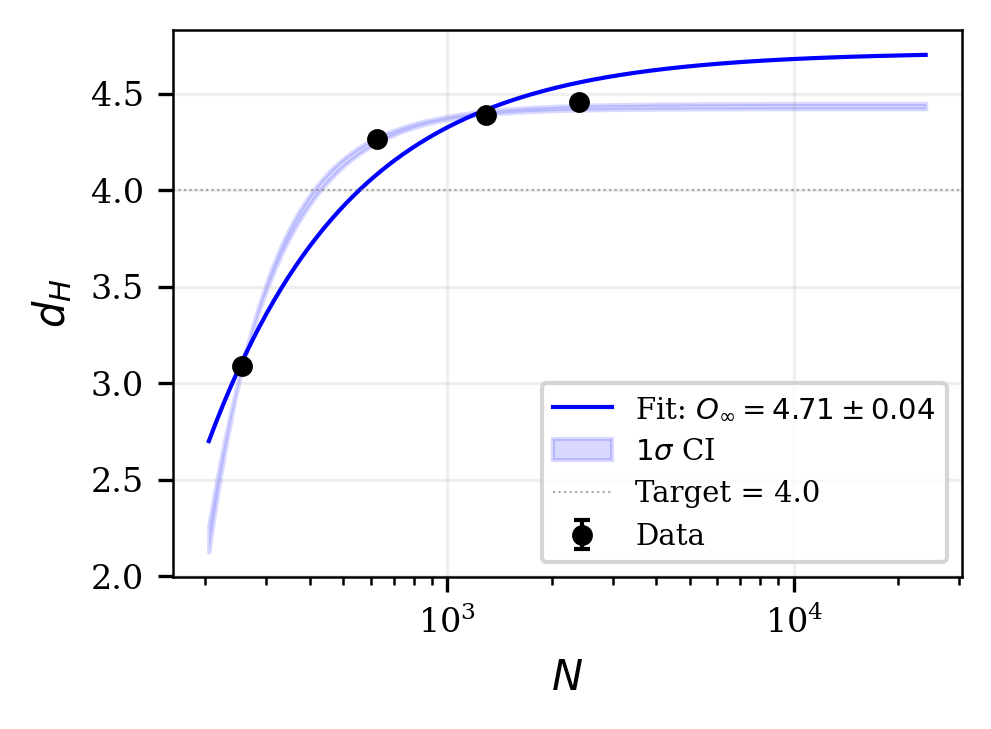
\includegraphics[width=\columnwidth]{fig6_scaling_dH.png}
  \caption{Hausdorff dimension $d_H$ vs.\ initial system size
    $N_0 = L^4$ (connected runs only).  Solid line: power-law
    fit~\eqref{eq:power_law} giving $d_H(\infty) = 4.71 \pm 0.04$.
    Shaded band: bootstrap 95\% CI.  Dashed line: target $d_H = 4$.
    The rightmost point is a single connected run out of 20.}
  \label{fig:scaling_dH}
\end{figure}

\subsection{Selection bias from connectivity conditioning}
\label{sec:selection_bias}

The decreasing connected fraction introduces a survivorship bias:
at large~$N$ we only measure geometry of the rare runs that
remain connected.  These ``survivors'' may not be representative.

At $L\!=\!8$, the single connected run may be an extreme
outlier, and its $d_H = 4.65$ should not be over-interpreted.
At $L\!=\!6$ and $L\!=\!7$, the 4--5 connected runs show low
scatter ($\sigma_{d_H} \approx 0.02$), suggesting some
regularity.  However, disconnected runs---which constitute the
majority at large $N$---have unknown $d_H$ because geometry
computations on the largest connected component are not performed.

A conservative interpretation is that the ``true'' large-$N$
behaviour of this rule is disconnection, and the extrapolated
$d_H^\infty = 4.71$ applies only to the increasingly rare
connected outliers.

\subsection{Spectral dimension at multiple scales}
\label{sec:spectral_multiscale}

Figure~\ref{fig:spectral_multiscale} shows the effective spectral
dimension $d_{\mathrm{eff}}(t) = -2\, d\!\ln P / d\!\ln t$ as a
function of diffusion time~$t$ for both the evolved graph and the
bare $5^4$ lattice (50\,000 walkers, 2000 steps).

The evolved graph showed a plateau at
$d_{\mathrm{eff}} \approx 0.74 \pm 0.03$ for $t \in [5, 117]$.
The bare lattice had a comparable plateau at
$d_{\mathrm{eff}} \approx 0.61 \pm 0.02$ for $t \in [26, 124]$.
Neither curve approached $d = 4$ within the accessible diffusion
times.

The key observation is that \textbf{evolution does not improve the
spectral dimension} relative to the bare lattice.  The evolved
and bare curves are indistinguishable within the measurement
uncertainty, indicating that the rule fails to create a diffusive
structure beyond what the initial lattice already possesses.

In CDT, Ambj{\o}rn~\emph{et al.}~\cite{Ambjorn2005} observe a
crossover from $d_s \approx 1.8$ at short diffusion times to
$d_s \approx 4$ at long times---a hallmark of UV-dimensional
reduction with correct IR geometry.  Our model shows no such
crossover: $d_{\mathrm{eff}}(t)$ remains flat and low at all
accessible scales (Fig.~\ref{fig:spectral_multiscale}).

We emphasise that this comparison has a caveat: the CDT result
is obtained at much larger effective volumes ($N \sim 10^5$)
where finite-size saturation is less severe.  The absence of a
crossover in our data may partly reflect the small graph sizes.
However, the bare lattice at $L\!=\!5$ already has 625 nodes,
and we see no hint of a rising $d_{\mathrm{eff}}$ even at
early times---suggesting a genuine structural limitation.

\begin{figure}[t]
  \centering
  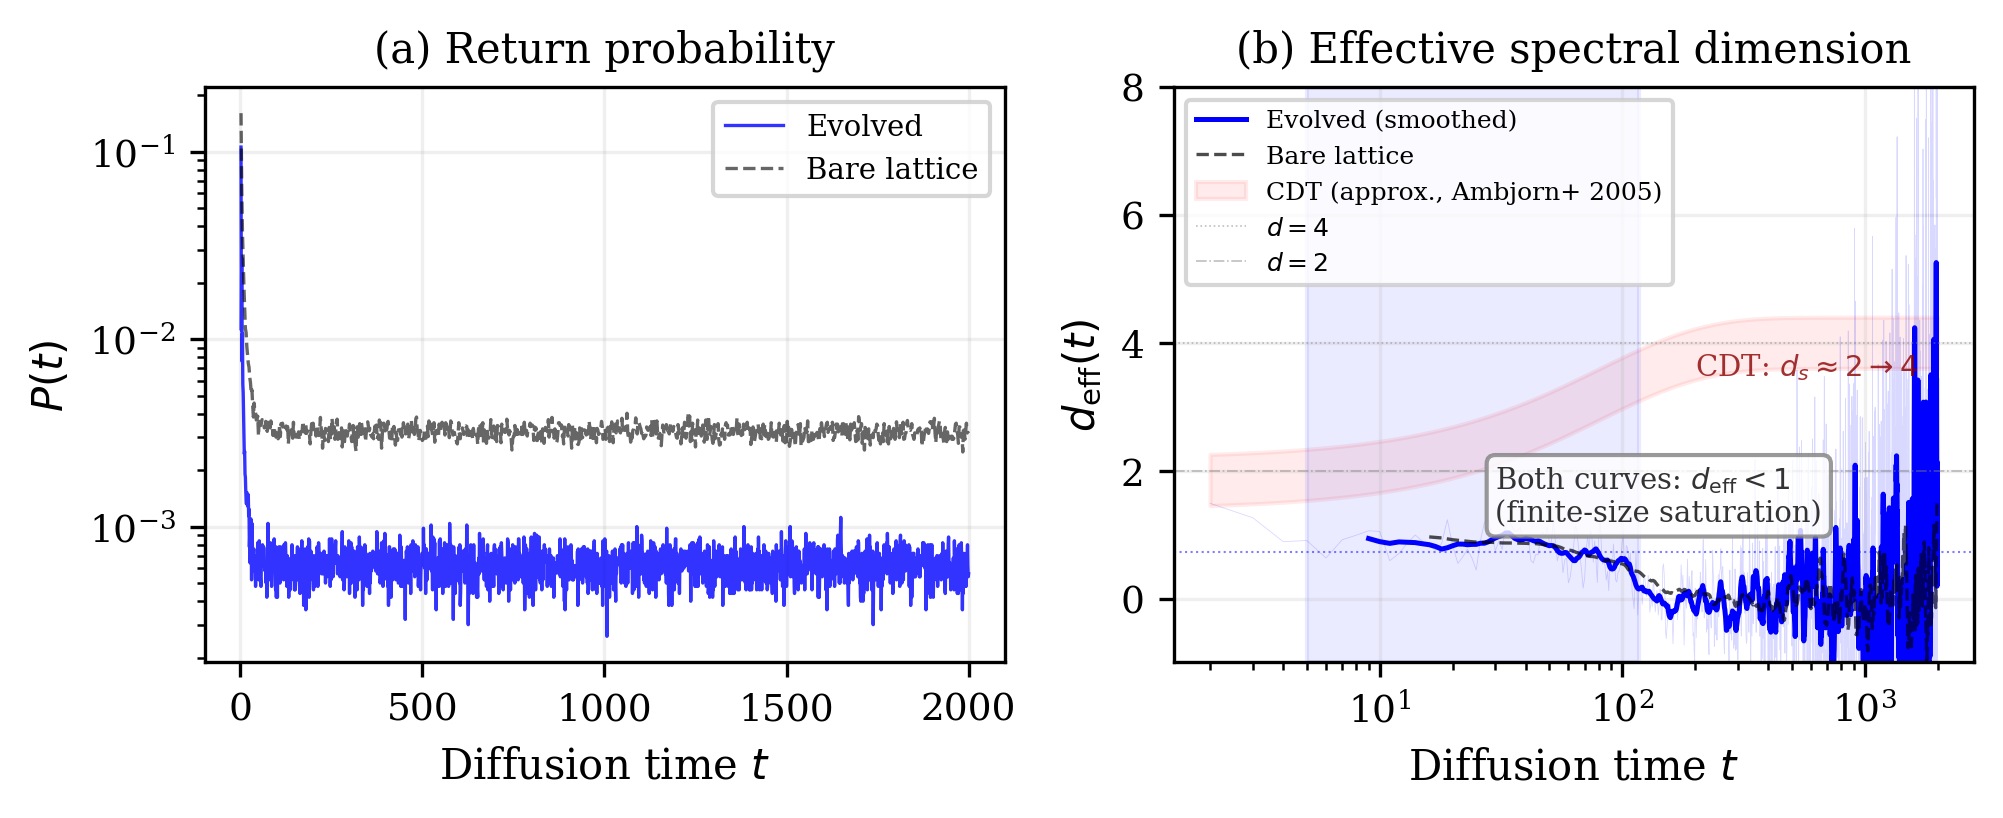
\includegraphics[width=\columnwidth]{fig9_spectral_multiscale.png}
  \caption{(a)~Return probability $P(t)$ for a single evolved graph
    and a bare $5^4$ lattice (50\,000 walkers each).
    (b)~Effective spectral dimension $d_{\mathrm{eff}}(t)$
    (smoothed, window = 15).  Red band: approximate CDT
    result~\cite{Ambjorn2005} (qualitative; CDT is measured at
    $N \sim 10^5$).  Neither evolved nor bare curve approaches
    $d = 4$.}
  \label{fig:spectral_multiscale}
\end{figure}

\subsection{Parameter--geometry correlations}
\label{sec:correlations}

To understand which parameters control the fitness, we analysed
the final GA population (40~individuals at generation~999) and
computed Pearson correlations between each parameter and total
fitness.

The topological parameters showed the strongest correlations:
$p_{\mathrm{add}}$ correlated positively ($r = +0.85$) and
$p_{\mathrm{mg}}$ negatively ($r = -0.63$) with fitness.
Among the 9~state-transition parameters, \emph{all} correlations
were $|r| < 0.3$, indicating that state dynamics played a negligible
role---the geometry was controlled almost entirely by the
topological moves.

The elite subset (top 20\% by fitness, 8~individuals) showed
extremely tight clustering in $p_{\mathrm{add}}$
($0.540 \pm 0.000$), suggesting a narrow, well-defined optimum.
This is consistent with the superiority of CMA-ES over GA:
CMA-ES excels at exploiting narrow optima in continuous
parameter spaces.


%% ════════════════════════════════════════════════════
\section{Discussion}
\label{sec:discussion}
%% ════════════════════════════════════════════════════

\subsection{Successes and failures}

The best rule demonstrates that metaheuristic optimisation can
navigate a 14-dimensional parameter space to find local dynamics
producing graphs with Hausdorff dimension in the correct range.
This is a non-trivial result: the vast majority of random
parameter choices yield disconnected or degenerate graphs.

However, three failures prevent us from claiming emergent
spacetime geometry:

\paragraph{1.~Connectivity instability.}
The rule fragments graphs with probability approaching unity
at $N > 2000$.  The evolved geometry does not persist in the
thermodynamic limit.  The rule was optimised at $N = 625$ and
exploits finite-size correlations that vanish at larger scales.
A multiscale training procedure, evaluating fitness at several
sizes simultaneously, might address this but would dramatically
increase computational cost.

\paragraph{2.~$d_H$ overshoot.}
The extrapolated $d_H(\infty) = 4.71$ exceeds the target by
18\%.  This is not ``approximately 4''---it reflects the
densification mechanism (node merging) that creates short-range
connections absent in a manifold triangulation.  The resulting
structure is intermediate between a 4-manifold and a
small-world network.  One might ask whether this is merely the
expected behaviour of any densification process on a hypercubic
lattice; we believe the answer is largely yes, which limits the
novelty of the $d_H$ result considered in isolation.

\paragraph{3.~Spectral dimension.}
The $d_s \approx 0.3$--$1$ values for evolved graphs are
comparable to those of the bare lattice at the same sizes.
While both are dominated by finite-size saturation (preventing
a definitive statement about the large-scale $d_s$), the
absence of \emph{any} improvement from evolution is a clear
negative signal: the rule does not create diffusive structure
beyond what the initial lattice already possesses.

\subsection{Hyperbolic curvature}

The curvature $\langle\kappa\rangle \to -0.34$ indicates
hyperbolic, not flat, emergent geometry.  This is consistent
with the general tendency of densified random graphs to have
negative Ollivier--Ricci curvature~\cite{Lin2011}: the merging
process creates geometry where the Wasserstein distance between
neighbourhood distributions exceeds the graph distance, yielding
$\kappa < 0$.

The convergence of $\langle\kappa\rangle$ to a finite value
in the $N \to \infty$ extrapolation is noteworthy: it suggests
a well-defined (if undesired) emergent geometry.  Whether this
hyperbolic space has cosmological relevance (as a discrete
analogue of anti-de Sitter space) is an interesting question
beyond the scope of this work.

\subsection{The role of causality}
\label{sec:causality}

Our results can be understood in the context of the EDT/CDT
dichotomy~\cite{Ambjorn2004,Ambjorn2012,Loll2019}.
Euclidean dynamical triangulations (without causal constraint)
produce either crumpled or branched-polymer phases---neither
of which has extended geometry.  CDT, with a foliation constraint
enforcing Lorentzian signature, produces four-dimensional
de~Sitter spacetime with $d_s \to 4$ in the IR.

Our model is analogous to EDT in that it imposes no causal
structure.  The cellular automaton rule applies symmetrically
in all graph directions; there is no preferred ``time'' direction,
no foliation, and no light-cone constraint.  The rule can
therefore create topological obstructions---bottlenecks, local
clusters connected by sparse bridges---that CDT's causal
constraint would prohibit.

Specifically, CDT's foliation prevents ``baby universes''
(spatial topology changes) which suppress diffusion by
trapping random walkers in disconnected
regions~\cite{Ambjorn2004}.  Our connectivity collapse at
large~$N$ is precisely this phenomenon: the acausal rule
allows the spatial topology to fragment.

This suggests that causal structure is not merely a
technical convenience but a \emph{necessary ingredient} for
emergent manifold-like geometry from discrete dynamics.
Our work provides computational support for this theoretical
expectation.

\subsection{Comparison with related approaches}

\paragraph{CDT.}
At comparable volumes, CDT achieves $d_s \approx 1.8$ (UV)
$\to 4$ (IR) and $d_H \approx 4$~\cite{Ambjorn2005}.  Our
model achieves $d_H \approx 4.7$ but no spectral crossover.
CDT operates at $N \sim 10^5$ simplices, roughly 25$\times$
our largest system.

\paragraph{Wolfram's physics project~\cite{Wolfram2020}.}
Hypergraph rewriting systems have been explored for emergent
spacetime but without published quantitative scaling results
comparable to CDT or this work.

\paragraph{Quantum graphity~\cite{Konopka2008}.}
Konopka~\emph{et al.}\ consider complete graphs with
dynamical edge states and observe a condensed phase with
geometric properties.  Our approach is complementary:
starting from a regular lattice (rather than a complete graph)
and using optimisation rather than statistical mechanics.
The connectivity collapse we observe may be analogous to their
``disordered'' (pre-geometric) phase.

\subsection{Limitations and future directions}

\begin{enumerate}
\item \textbf{Graph size.}  $N \le 4096$ limits the scaling
  analysis.  Larger systems ($N \sim 10^5$) would reduce
  finite-size effects on all observables, especially $d_s$.

\item \textbf{Parameter space.}  The 14-parameter rule may be
  insufficiently expressive.  Richer rule classes---e.g.\
  with memory, non-local awareness, or adaptive
  parameters---might explore a wider space of emergent
  geometries.

\item \textbf{Spectral dimension estimator.}  At accessible
  sizes, $d_s$ is dominated by saturation.  Alternative
  spectral probes (e.g.\ graph Laplacian eigenvalues) may be
  more informative at small~$N$.

\item \textbf{Single-scale training.}  The rule was optimised
  at a single size ($N = 625$).  Multiscale fitness
  evaluation could enforce scale-invariance.

\item \textbf{Causality.}  The most important extension would
  be to incorporate causal structure---e.g.\ a preferred
  time direction with a foliation constraint or a partial
  order on nodes---and repeat the search.  If such a
  ``causal discrete automaton'' achieves $d_s \to 4$, it
  would provide strong evidence for the necessity of
  causality in discrete quantum gravity.

\item \textbf{Fitness function.}  Adding a direct $|d_H - 4|$
  penalty and a connected-component penalty that scales
  more aggressively might yield better-behaved rules,
  though at the risk of fine-tuning.
\end{enumerate}


%% ════════════════════════════════════════════════════
\section{Conclusions}
\label{sec:conclusions}
%% ════════════════════════════════════════════════════

We have presented \textsc{Discretum}, a computational framework
for searching cellular automaton rules on dynamic graphs that
produce emergent geometry.  Applying CMA-ES and genetic algorithm
optimisation to a 14-parameter rule on four-dimensional hypercubic
lattices, we find that:

\begin{enumerate}
\item The best rule produces graphs with Hausdorff dimension
  $d_H = 3.09$--$4.65$ increasing with system size, extrapolating
  to $d_H(\infty) = 4.71 \pm 0.04$---systematically above the
  target $d_H = 4$.

\item Connectivity degrades from 100\% at $N = 256$ to 5\% at
  $N = 4096$.  The rule is not thermodynamically stable.

\item The spectral dimension $d_s \lesssim 1$ is not improved
  relative to the bare lattice, indicating no emergent diffusive
  structure.  This observable is, however, strongly affected by
  finite-size saturation at $N \le 4096$.

\item The Ollivier--Ricci curvature converges to
  $\langle\kappa\rangle = -0.34 \pm 0.006$: hyperbolic, not flat.

\item The topological moves (edge addition, node merging)
  dominate the fitness landscape; the 9~state-transition
  parameters are essentially irrelevant.
\end{enumerate}

These results demonstrate that 14-parameter acausal local rules
on dynamic graphs can achieve the correct volume growth scaling
($d_H$) but fail to produce manifold-like diffusion ($d_s$),
flat curvature ($\kappa \to 0$), or thermodynamic stability.
The comparison with CDT---where imposing causal structure
produces all of these properties---provides computational
evidence that causality is a necessary ingredient for emergent
spacetime geometry, consistent with the EDT/CDT dichotomy.

The framework, including GPU-accelerated Ollivier--Ricci
computation, CMA-ES/GA optimisation, ensemble diagnostics,
spectral analysis, and finite-size scaling tools, is released
as open-source software~\cite{discretum_code} to facilitate
further exploration of discrete quantum gravity models.

\begin{acknowledgments}
This research received no external funding and was conducted
independently.  The author declares no competing interests.
Computations were performed on an Intel Core i7-12700F with
64\,GB DDR5 and an AMD Radeon RX\,7900\,XTX GPU using
HIP/ROCm~7.2.
\end{acknowledgments}

\appendix

\section{Code and data availability}
\label{sec:code}

The \textsc{Discretum} code is available at
\url{https://github.com/mnarc123/discretum}
under the MIT licence.

The repository includes:
\begin{itemize}
\item Complete C++20/HIP source code with CMake build system
\item Unit test suite (679~assertions, 39~test cases)
\item GPU kernels for AMD ROCm (tested on RX\,7900\,XTX)
\item Python analysis scripts for all figures in this paper
\item Reproduction script (\texttt{scripts/reproduce.sh})
  regenerating all results and figures from source
\item Configuration files for all search campaigns
\item Raw data from scaling analysis
  (\texttt{data/results/scaling\_4d\_v3/})
\end{itemize}

Build and test:
\begin{verbatim}
cmake -B build -G Ninja
ninja -C build
./build/tests           # 679 assertions
./build/discretum_validate # 7 checks
\end{verbatim}

\bibliography{references}

\end{document}
